\documentclass[]{exam}

%These tell TeX which packages to use.
\usepackage{array,epsfig}
\usepackage{amsmath}
\usepackage{amsfonts}
\usepackage{amssymb}
\usepackage{amsxtra}
\usepackage{amsthm}
\usepackage{mathrsfs}
\usepackage[dvipsnames]{xcolor}
\usepackage{array}
\usepackage{graphicx}
\graphicspath{ {../art/} }
\usepackage{bm}
\usepackage{tikz}
\usepackage{multicol}
\usepackage{enumitem}

\renewcommand\qedsymbol{$\blacksquare$}

%Here I define some theorem styles and shortcut commands for symbols I use often
\theoremstyle{definition}
\newtheorem{defn}{Definition}
\newtheorem{thm}{Theorem}
\newtheorem{cor}{Corollary}
\newtheorem*{rmk}{Remark}
\newtheorem{lem}{Lemma}
\newtheorem*{joke}{Joke}
\newtheorem{ex}{Example}
\newtheorem*{soln}{Solution}
\newtheorem{prop}{Proposition}

\newcommand{\lra}{\longrightarrow}
\newcommand{\ra}{\rightarrow}
\newcommand{\surj}{\twoheadrightarrow}
\newcommand{\graph}{\mathrm{graph}}
\newcommand{\bb}[1]{\mathbb{#1}}
\newcommand{\Ell}{\mathscr{L}}
\newcommand{\Z}{\bb{Z}}
\newcommand{\Q}{\bb{Q}}
\newcommand{\R}{\bb{R}}
\newcommand{\C}{\bb{C}}
\newcommand{\N}{\bb{N}}
\newcommand{\M}{\mathbf{M}}
\newcommand{\m}{\mathbf{m}}
\newcommand{\MM}{\mathscr{M}}
\newcommand{\HH}{\mathscr{H}}
\newcommand{\Om}{\Omega}
\newcommand{\Ho}{\in\HH(\Om)}
\newcommand{\bd}{\partial}
\newcommand{\del}{\partial}
\newcommand{\bardel}{\overline\partial}
\newcommand{\textdf}[1]{\textbf{\textsf{#1}}\index{#1}}
\newcommand{\img}{\mathrm{img}}
\newcommand{\ip}[2]{\left\langle{#1},{#2}\right\rangle}
\newcommand{\inter}[1]{\mathrm{int}{#1}}
\newcommand{\exter}[1]{\mathrm{ext}{#1}}
\newcommand{\cl}[1]{\mathrm{cl}{#1}}
\newcommand{\ds}{\displaystyle}
\newcommand{\vol}{\mathrm{vol}}
\newcommand{\cnt}{\mathrm{ct}}
\newcommand{\osc}{\mathrm{osc}}
\newcommand{\LL}{\mathbf{L}}
\newcommand{\UU}{\mathbf{U}}
\newcommand{\support}{\mathrm{support}}
\newcommand{\AND}{\;\wedge\;}
\newcommand{\OR}{\;\vee\;}
\newcommand{\Oset}{\varnothing}
\newcommand{\st}{\ni}
\newcommand{\wh}{\widehat}

%Pagination stuff.
\setlength{\topmargin}{-.3 in}
\setlength{\oddsidemargin}{0in}
\setlength{\evensidemargin}{0in}
\setlength{\textheight}{9.in}
\setlength{\textwidth}{6.5in}

\newcommand{\id}[1]{\mbox{\it #1\/}}
\newcommand{\rid}[1]{\mbox{\rm #1}}
\newcommand{\sid}[1]{\mbox{\sf #1}}
\newcommand{\bid}[1]{\mbox{\bf #1}}
\newcommand{\tinysz}[1]{\mbox{\tiny $#1$}}



\newcommand{\twonode}{%
  \begingroup\normalfont
  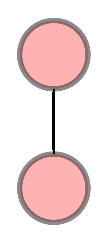
\includegraphics[height=\fontcharht\font`\b]{2nodetree.eps}%
  \endgroup
}


\title{Lab 3: The Weak, the Strong and the Mutual}
\author{Foundations of Computer Science}
\date{\today}
%\pagestyle{empty} 
%\footer{}{\thepage}{}

\noprintanswers
\unframedsolutions
\SolutionEmphasis{\itshape\small}
\SolutionEmphasis{\color{NavyBlue}}


\begin{document}

\maketitle

\setlength{\columnseprule}{1pt}
\begin{questions}


\question Consider the following recursive definitions of sets of strings. 
For each of the definitions given, choose the induction rule most suitable 
for proving properties of the system defined:
\begin{multicols}{2}
{\bf Recursive Definitions:}\\
\begin{enumerate}
\item
\begin{tabbing}
{\bf R2}XX \=  \kill
{\bf B1} \>
        \(\begin{array}[t]{l}
        a \in S
        \end{array}\) \\[2ex]
{\bf B2} \>
        \(\begin{array}[t]{l}
        b \in S
        \end{array}\) \\[2ex]
{\bf R} \>
        \(\begin{array}[t]{l}
        x \in S \;\;\;y \in S \\
        \hline
        xy \in S
        \end{array}\)
\end{tabbing}
\hrule
\item
\begin{tabbing}
{\bf R2}XX \=  \kill
{\bf B} \>
        \(\begin{array}[t]{l}
        a \in S
        \end{array}\) \\[2ex]
{\bf R} \>
        \(\begin{array}[t]{l}
        x \in S \;\;\;y \in S \\
        \hline
        xy \in S
        \end{array}\)
\end{tabbing}
\hrule

\item
\begin{tabbing}
{\bf R2}XX \=  \kill
{\bf B} \>
        \(\begin{array}[t]{l}
        a \in S
        \end{array}\) \\[2ex]
{\bf R} \>
        \(\begin{array}[t]{l}
        x \in S \\
        \hline
        xbx \in S
        \end{array}\)
\end{tabbing}
\end{enumerate}

\columnbreak
{\bf Induction Rules:}\\
\begin{tabbing}
[1]XX \=  \kill
[1] \>
	\(\begin{array}[t]{l}
	S(i) \;\wedge\; \forall n \geq i.\;S(n) \Rightarrow S(n+1) \\
	\hline
	\forall n \geq i. \; S(n)
	\end{array}\) % \\[2ex]
\end{tabbing}

\begin{tabbing}
[2]XX \=  \kill
[2] \>
	\(\begin{array}[t]{l}
	S(i) \;\wedge\; \forall n \geq i.\;S(i)\;\wedge\;S(i+1)\;\wedge\cdots\wedge\;S(n) \Rightarrow S(n+1) \\
	\hline
	\forall n \geq i. \; S(n)
	\end{array}\)
\end{tabbing}

\begin{tabbing}
[3]XX \=  \kill
[3] \>
	\(\begin{array}[t]{l}
	S(i) \;\wedge\; S(i+1)\;\wedge\cdots\wedge\;S(j)\;\wedge\; \\
\forall n \geq j.\;S(i)\;\wedge\;S(i+1)\;\wedge\cdots\wedge\;S(n) \Rightarrow S(n+1) \\
	\hline
	\forall n \geq i. \; S(n)
	\end{array}\) % \\[2ex]
\end{tabbing}
~\\
~\\
~\\
~\\
    
\end{multicols}
\begin{solution}
Note that the question asks for the ``most suitable'' rule given
the structure of the system, but to choose a definitive answer you would need to
also be given the property that you are proving. With this caveat, reasonable
choices are rule [3] or [2] for system $1$, rule [3] or [2] for system $2$, and 
rule [1] (weak induction) for system $3$. 
\end{solution}

\question What is the meaning of $j$ in the third induction rule? What does it
represent, and what determines its value relative to $i$?
\begin{solution}
$j$ represents the index of the last base case. If there are
$b$ base cases, the value of $j$ will be $i + b - 1$.
\end{solution}


\question Referencing the definition of rooted trees given in the slides,
draw the structure produced in the following derivation:
\begin{center}
\begin{tabular}{lllll}
  $\bid{B}$  & $\id{nil}\in\id{RTL}$            &                       & &
  \\ \cline{2-2} 
  $\bid{R2}$ & $\id{node}(\id{nil})\in\id{RT}$  & $\id{nil}\in\id{RTL}$ & $\bid{B}$ &
  \\ \cline{2-3}
  $\bid{R1}$ & \multicolumn{2}{l}{ $\id{cons}(\id{node}(\id{nil}),\id{nil})\in\id{RTL}$} & & 
  \\ \cline{2-3}
  $\bid{R2}$ & \multicolumn{2}{l}{ $\id{node}(\id{cons}(\id{node}(\id{nil}),\id{nil}))\in\id{RT}$} & $\id{nil} \in \id{RTL}$ & $\bid{B}$
  \\ \cline{2-4}
  $\bid{R1}$ &
  \multicolumn{3}{l}{$\id{cons}(\id{node}(\id{cons}(\id{node}(\id{nil}),\id{nil})), \id{nil})\in\id{RTL}$}
\end{tabular}
\end{center}
\begin{solution}
$[\twonode]$
\end{solution}

\question What is the derivation height of the following tree:  

\begin{center}
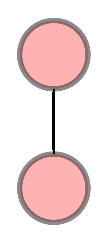
\includegraphics[height=2cm]{2nodetree.eps}%
\end{center}
\begin{solution}
3
\end{solution}

\question Reproduced below is the argument from slide $6$ of the mutual
induction slide set, which proves that the number of edges in a rooted
tree list, $l'$, of derivation height $n + 1$ is equal to the number of nodes
in the list, minus the length of the list. Work through each of the
steps below and annotate each line by adding a plain-language explanation as to 
why it follows from the line above. (Feel free to reference the original slides
as needed).

\begin{displaymath}
\begin{array}{llll}
1. & \id{\#edges}(l') & = &\id{\#edges}(\id{cons}(t,l)) \\
2. &  & = & \id{\#edges}(t) + \id{\#edges}(l) \\
3. & 	& = & \id{\#nodes}(t) - 1 + \id{\#edges}(l) \\
4. & 	& = & \id{\#nodes}(t) - 1 + \id{\#nodes}(l) - |l| \\
5. & 	& = & \id{\#nodes}(\id{cons}(t,l)) - 1 - |l| \\
6. & 	& = & \id{\#nodes}(\id{cons}(t,l)) - (1 + |l|) \\
7. & 	& = & \id{\#nodes}(\id{cons}(t,l)) - |\id{cons}(t,l)|\\
8. & 	& = & \id{\#nodes}(l') - |l'|
\end{array}
\end{displaymath}


% MAYBE NEXT WEEK
%
%Recall that a ``leaf'' node is a node with no children
%and an ``internal'' node is a node with children.
%
%Recall that a full binary tree is one in which each internal
%node has exactly two children.
%
%Write a Post System for full binary trees.
%
%Let L be the number of ``leaf'' nodes and I be the number of internal nodes.
%Prove that, for all full binary trees, L = I + 1.



\end{questions}
\end{document}


